\begin{name}
	{\tenchude}
	{TOÁN 10}
	{LỚP TOÁN THẦY PHÁT}
	{{Không biết thì không có gì xấu hổ.\\ Chỉ nên cảm thấy xấu hổ khi không chịu học hỏi.}}
\end{name}
\TN
\begin{ex}%[0D6N3-3]
Cân nặng (kg) của một nhóm học sinh nữ lớp $10$A cho bởi số liệu sau:
\[
\begin{array}{llllllllll}
38 & 39 & 44 & 44 & 46 & 47 & 47 & 48 & 52 & 55.
\end{array}
\]
Tìm số trung vị của mẫu số liệu trên.
\choice
{$44$}
{$46$}
{\True $46{,}5$}
{$47$}
\loigiai{
Dãy trên đã sắp xếp không giảm, và có $10$ số trong mẫu số liệu.\\
Số liệu thứ $5$ là $46$ và số liệu thứ $6$ là $47$.\\
Vậy số trung vị là $M_e=\dfrac{46+47}{2}=46{,}5$.}
\end{ex}

\begin{ex}%[0-HK1-CT-4-THTHDHSG-HCM-2324]%[VN-MT-6, VM026]%[0D6N4-2]
Khoảng biến thiên của mẫu số liệu $8$; $7$; $6$; $5$; $8$; $1$; $4$; $5$ là
\choice
{$6$}
{\True $7$}
{$3$}
{$4$}
\loigiai{
Khoảng biến thiên của mẫu số liệu là $8-1=7$.
}
\end{ex}

\begin{ex}%[0D8H1-3]
Từ các chữ số $1$, $2$, $3$, $4$, $5$ có thể lập được bao nhiêu số tự nhiên bé hơn $60$?
\choice
{$42$}
{\True $30$}
{$25$}
{$17$}
\loigiai{
\begin{itemize}
\item Số cần tìm có $1$ chữ số $\Rightarrow$ có $5$ số thỏa mãn yêu cầu.
\item Số cần tìm có $2$ chữ số $\Rightarrow$ có $5\cdot 5=25$ số thỏa mãn yêu cầu.
\end{itemize}
Vậy có $5+25=30$ (số thỏa mãn yêu cầu).
}
\end{ex}

\begin{ex}%[0D8H2-3]
Cho tập $A=\left\{{0,1, 2,\ldots ,9}\right\}.$ Số các số tự nhiên có $5$ chữ số đôi một khác nhau lấy ra từ tập $ A$ là?
\choice
{$30420$}
{$27162$}
{\True $27216$}
{$30240$}
\loigiai{
Gọi số cần tìm là $\overline{abcde},\,a\ne 0$.\\
$\bullet $ Chọn $ a$ có 9 cách.\\
$\bullet $ Chọn $ b,\,c,\,d,\,e$ từ 9 số còn lại có $ \mathrm{A}_9^4=3024$ cách.\\
Vậy có $ 9\cdot 3024=27216$.}
\end{ex}

\begin{ex}%[BG - 10 New - 4in1,Phan Chiến Thắng]%[0D8H2-4]
Sắp xếp năm bạn học sinh An, Bình, Chi, Dũng, Lệ vào một chiếc ghế dài có $5$ chỗ ngồi. Số cách sắp xếp sao cho bạn Chi luôn ngồi chính giữa là
\choice
{$16$}
{$120$}
{$60$}
{\True $24$}
\loigiai{
Xếp bạn Chi ngồi giữa có $1$ cách. Số cách xếp $4$ bạn sinh An, Bình, Dũng, Lệ vào $4$ chỗ còn lại là số hoán vị của $4$ phần tử nên có có $4!$ cách. Vậy có $24$ cách xếp.
}
\end{ex}

\begin{ex}%[0D8H2-6]
Cho hai đường thẳng song song $d_1$ và $d_2.$ Trên $d_1$ lấy $17$ điểm phân biệt, trên $d_2$ lầy $20$ điểm phân biệt. Tính số tam giác mà có các đỉnh được chọn từ $37$ điểm này.
\choice
{$5690$}
{$5960$}
{\True $5950$}
{$5590$}
\loigiai{
Một tam giác được tạo bởi ba điểm phân biệt nên ta xét
\begin{itemize}
\item \textbf{TH1:} Chọn $1$ điểm thuộc $d_1$ và $2$ điểm thuộc có $\mathrm{C}_{17}^1\cdot\mathrm{C}_{20}^2$ tam giác.
\item \textbf{TH2:} Chọn $2$ điểm thuộc $d_1$ và $1$ điểm thuộc có $\mathrm{C}_{17}^2\cdot\mathrm{C}_{20}^1$ tam giác.
\end{itemize}
Như vậy, ta có $\mathrm{C}_{17}^1\cdot \mathrm{C}_{20}^2+\mathrm{C}_{17}^2\cdot\mathrm{C}_{20}^1=5950$ tam giác cần tìm.}
\end{ex}

\begin{ex}%[0D8H3-2]
Khai triển nhị thức $P\left(a\right)=\left(a-1\right)^7$ theo số mũ tăng dần của $a$
\choice
{\True $P\left(a\right)=-1+7a-21a^2+35a^3-35a^4+21a^5-7a^6+a^7$}
{$P\left(a\right)=1+7a+21a^2+35a^3+35a^4+21a^5+7a^6+a^7$}
{$P\left(a\right)=a^7-7a^6+21a^5-35a^4+35a^3-21a^2+7a-1$}
{$P\left(a\right)=-1+7a-21a^2+30a^3-35a^4+21a^5-7a^6+a^7$}
\loigiai{
Ta có
\begin{align*}
P\left(a\right)	&=\left(-1+a\right)^7=-\mathrm{C}_7^0+\mathrm{C}_7^1a-\mathrm{C}_7^2a^2+\mathrm{C}_7^3a^3-\mathrm{C}_7^4a^4+\mathrm{C}_7^5a^5-\mathrm{C}_7^6a^6+\mathrm{C}_7^7a^7  \\
&=-1+7a-21a^2+35a^3-35a^4+21a^5-7a^6+a^7.
\end{align*}
}
\end{ex}

\begin{ex}%[10-11-EX-GHK2-2425]%[Lê Toàn]%[0H9H1-2]
Trong mặt phẳng $Oxy$, cho $\overrightarrow{a}=(-2; 1)$, $\overrightarrow{b}=(3;-2)$. Tìm tọa độ véc-tơ $\overrightarrow{x}$ thỏa biểu thức $\overrightarrow{x}=-3\overrightarrow{a}+2\overrightarrow{b}$.
\choice
{\True $\overrightarrow{x}=(12;-7)$}
{$\overrightarrow{x}=(0;-7)$}
{$\overrightarrow{x}=(12;1)$}
{$\overrightarrow{x}=(0;1)$}
\loigiai{
Ta có $-3\overrightarrow{a}=(6;-3)$, $2\overrightarrow{b}=(6;-4)$.\\
Vậy $\overrightarrow{x}=-3\overrightarrow{a}+2\overrightarrow{b}=(12;-7)$.
}
\end{ex}

\begin{ex}%[0H9H3-2]
Phương trình tham số của đường thẳng đi qua hai điểm $A\left( 2;-1 \right)$ và $B\left( 2;5 \right)$ là
\choice
{$\heva{
& x=2t \\
& y=-6t
}$}
{$\heva{
& x=2+t \\
& y=5+6t
}$}
{$\heva{
& x=1 \\
& y=2+6t \\
}$}
{\True $\heva{
& x=2 \\
& y=-1+6t
}$}
\loigiai{
Véc-tơ chỉ phương $\vec{AB}=\left( 0;6 \right)$.\\
Phương trình đường thẳng $AB$ đi qua $A$ và có véc-tơ chỉ phương $\vec{AB}=\left( 0;6 \right)$ là $\heva{
& x=2 \\
& y=-1+6t.
}$
}
\end{ex}

\begin{ex}%[0H9H4-2]%[Tex hóa đề CK2 - form 2025 - đọt 2 -Huỳnh Thanh Chí]
Cho 2 điểm $A(1; 1), B(7; 5)$. Phương trình đường tròn đường kính $AB$ là
\choice
{\True $x^2+y^2-8x-6y+12=0$}
{$x^2+y^2+8x+6y-12=0$}
{$x^2+y^2+8x+6y+12=0$}
{$x^2+y^2-8x-6y-12=0$}
\loigiai{Ta có tâm $I$ là trung điểm của đoạn thẳng $AB$ và bán kính $R=\dfrac{AB}{2}$.\\
Suy ra $\heva{&x_I=\dfrac{x_A+x_B}{2} \\
&y_I=\dfrac{y_A+y_B}{2}} \Rightarrow\heva{&x_I=\dfrac{1+7}{2}=4\\
&y_I=\dfrac{1+5}{2}=3} \Rightarrow I=(4; 3)$.\\
$R=\dfrac{AB}{2}=\dfrac{\sqrt{(7-1)^2+(5-1)^2}}{2}=\sqrt{13}$.\\
Phương trình đường tròn đường kính $AB$ là\\
$(x-4)^2+(y-3)^2=(\sqrt{13})^2\Leftrightarrow x^2+y^2-8x-6y+12=0$.\\
Kết luận phương trình đường tròn đường kính $AB$ là $x^2+y^2-8x-6y+12=0$.
}
\end{ex}

\begin{ex}%[0H9H5-2]%[Dự án đề kiểm tra Toán 11 GHKII NH23-24-Nguyen Tran Anh Tuan]%[THPT Thiệu Hóa - Thanh Hóa]
Elip có độ dài trục nhỏ là $4\sqrt{6}$ và có một tiêu điểm $F(5; 0)$. Phương trình chính tắc của elip là
\choice
{\True $\dfrac{x^2}{49}+\dfrac{y^2}{24}=1$}
{$\dfrac{x^2}{29}+\dfrac{y^2}{24}=1$}
{$\dfrac{x^2}{101}+\dfrac{y^2}{96}=1$}
{$\dfrac{x^2}{121}+\dfrac{y^2}{96}=1$}
\loigiai{
Elip $(E)$ có độ dài trục nhỏ là $4\sqrt{6} \Rightarrow 2b=4\sqrt{6} \Rightarrow b=2\sqrt{6}$.\\
Elip $(E)$ có một tiêu điểm $F(5; 0) \Rightarrow c=5$. Khi đó, $a=\sqrt{b^2+c^2}=7$.\\
Phương trình chính tắc của Elip là $(E)\colon \dfrac{x^2}{49}+\dfrac{y^2}{24}=1$.
}
\end{ex}

\begin{ex}%[0H9H5-4]%[Dự án đề kiểm tra Toán khối 11 HKII NH23-24-Dot15-PhucChuong]%[THPT Nhu Van Lang - Hai Phong]
Đường Hypebol $\dfrac{x^2}{16}-\dfrac{y^2}{9}=1$ có một tiêu điểm là điểm nào dưới đây?
\choice
{$\left(0;5\right)$}
{\True$\left(-5;0\right)$}
{$\left(\sqrt{7};0\right)$}
{$\left(0;\sqrt{7}\right)$}
\loigiai{
Đường Hypebol $\dfrac{x^2}{16}-\dfrac{y^2}{9}=1$ có hai tiêu điểm là $F_1(-5;0)$ và $F_2(5;0)$.
}
\end{ex}
\TNTF
\begin{ex}%[0D8H2-4]%[0D4K2-4]
Một nhóm có $14$ người trong đó có hai bạn tên An và Bình. Người ta cần chọn một tổ công tác gồm $6$ người từ nhóm $14$ người đó.
\choiceTF
{\True Số cách chọn một nhóm $6$ người bất kỳ là $3\,003$ cách}
{\True Số cách chọn một nhóm $6$ người trong đó không có An và Bình là $924$ cách}
{\True Số cách chọn một nhóm $6$ người trong đó có $1$ tổ trưởng, $5$ tổ viên và chỉ có một trong hai người An hoặc Bình là $9\,504$ cách}
{Số cách chọn một nhóm $6$ người trong đó có mặt cả An và Bình là $1\,848$ cách}
\loigiai{
\begin{itemchoice}
\itemch \textbf{Đúng}.\\
Mỗi cách chọn một nhóm $6$ người bất kỳ là một tổ hợp chập $6$ của $14$ phần tử.\\
Vậy có $\mathrm{C}_{14}^6=3\,003$ cách chọn.
\itemch \textbf{Đúng}.\\
Mỗi cách chọn một nhóm $6$ người mà không có mặt An và Bình là một tổ hợp chập $6$ của $12$.\\
Vậy có $\mathrm{C}_{12}^6=924$ cách chọn.
\itemch \textbf{Đúng}. \\
- Chọn một nhóm $6$ người có An nhưng không có Bình, có $\mathrm{C}_{12}^5 = 792$ cách.\\
- Chọn một nhóm $6$ người có Bình nhưng không có An, có $\mathrm{C}_{12}^5 = 792$ cách.\\
- Từ nhóm $6$ người chọn ra, chọn $1$ người làm tổ trưởng, có $6$ cách chọn.\\
Vậy có $2\cdot 792 \cdot 6 = 9\,504$ cách chọn thỏa yêu cầu bài toán.
\itemch \textbf{Sai}. \\
- Chọn An và Bình sau đó chọn $4$ người từ $12$ người còn lại. Số cách chọn là  $\mathrm{C}_{12}^4=495$ cách chọn.
\end{itemchoice}
}
\end{ex}

\begin{ex}%[Dự án 18 - TeamTeXHoa - Phạm Quốc Toàn]%[0H9H4-5]
Trong mặt phẳng tọa độ $Oxy$, cho hai điểm $A \left(1;-4 \right)$, $B \left(-2;0 \right)$ và đường thẳng \\
$d \colon 2x-4y+1=0$. Các mệnh đề sau đúng hay sai?
\choiceTF
{Điểm $A$, $B$ cách đều đường thẳng $d$}
{Tọa độ tâm của đường tròn đi qua hai điểm $A$, $B$ và có tâm thuộc đường thẳng $d$ là $I \left(1;\dfrac{3}{4}\right)$}
{\True Phương trình đường tròn $\left(C \right)$ đi qua $A$, $B$ và có tâm thuộc đường thẳng $d$ là \\
$4x^2+4y^2-60x-32y-136=0$}
{\True Giá trị nhỏ nhất của $OM$ với $M$ là điểm chuyển động trên đường tròn là $\dfrac{5\sqrt{17}-17}{2}$}
\loigiai{
\begin{itemchoice}
\itemch Khoảng cách từ điểm $A$ đến đường thẳng $d$ là $d\left(A, d\right)=\dfrac{\left| 2\cdot 1-4 \cdot \left(-4 \right)+1\right|}{\sqrt{2^2+ \left(-4 \right)^2}}=\dfrac{19\sqrt{5}}{10}$. \\
Khoảng cách từ điểm $B$ đến đường thẳng $d$ là $d\left(B, d\right)=\dfrac{\left| 2\cdot \left(-2 \right)-4 \cdot 0 +1\right|}{\sqrt{2^2+ \left(-4 \right)^2}}=\dfrac{3\sqrt{5}}{10}$. \\
Vậy hai điểm $A$, $B$ không cách đều đường thẳng $d$.
\itemch Đường tròn có tâm thuộc đường thẳng $d \colon 2x-4y+1=0$ nên gọi $I$ là tâm đường tròn thì $I\left(2a-\dfrac{1}{2};a\right)$.\\
Mặt khác đường tròn đi qua $A$, $B$ nên $IA=IB\Leftrightarrow \left| \overrightarrow{IA}\right|=\left| \overrightarrow{IB}\right|$ \\
$\Leftrightarrow \sqrt{\left(1-2a+\dfrac{1}{2}\right)^2+ \left(-4-a \right)^2}=\sqrt{\left(-2-2a+\dfrac{1}{2}\right)^2+ \left(0-a \right)^2}\Leftrightarrow a=4$. \\
Vậy đường tròn đi qua $A$, $B$ và có tâm thuộc đường thẳng $d$ có tọa độ tâm là $I\left(\dfrac{15}{2};4\right)$.
\itemch $R=IB=\left| \overrightarrow{IB}\right|=\sqrt{\left(-2-\dfrac{15}{2}\right)^2+ \left(0-4 \right)^2}=\dfrac{5\sqrt{17}}{2}$. \\
Phương trình đường tròn đi qua $A$, $B$ và có tâm thuộc đường thẳng $d$ là \\
$\left(x-\dfrac{15}{2}\right)^2+ \left(y-4 \right)^2=\left(\dfrac{5\sqrt{17}}{2}\right)^2 \Leftrightarrow 4x^2+4y^2-60x-32y-136=0$.
\itemch Gọi $G$, $K$ lần lượt là giao điểm của đường thẳng $IO$ và đường tròn.
\begin{center}
\begin{tikzpicture}[>=stealth, x=1.0 cm, y=1.0 cm]
\draw[->] (-3,0) --(0,0) node[below right]{$O$} -- (4,0) node[below]{$x$};
\draw[->](0,-3)--(0, 4.5) node[right]{$y$};
\draw(1,1) circle (3); %(0,0) là tọa độ tâm, 1 là bán kính
\draw(1,1) -- (-1.12, -1.12) (1, 1) -- (3.11, 3.13) (0, 0) -- (1, 4) -- (1, 1);
\draw (1,1) circle (1pt) node[below]{$I$};
\draw (1,4) circle (1pt) node[above]{$M$};
\draw (-1.12, -1.12) circle (1pt) node[below left]{$G$};
\draw (3.11, 3.13) circle (1pt) node[above right]{$K$};
\end{tikzpicture}
\end{center}
Với ba điểm $I$, $O$, $M$ ta có \\
$IM-IO \le OM \le IM+IO \Rightarrow IG-IO \le OM \le IK+IO \Rightarrow OG \le OM \le OK$. \\
Trong đó $OG=IG-IO=\dfrac{5\sqrt{17}}{2}-\dfrac{17}{2}=\dfrac{5\sqrt{17}-17}{2}$. \\
Vậy $OM$ đạt giá trị nhỏ nhất là $\dfrac{5\sqrt{17}-17}{2}$ khi $M$ trùng $G$.
\end{itemchoice}
}
\end{ex}
\TNSA
\begin{ex}%[Chuẩn hóa M25, Nguyễn Văn Nay]%[0D0V2-5]
Một hộp có $12$ quả bóng khác nhau; trong đó có $5$ quả màu đỏ, $4$ quả màu vàng, $3$ quả màu xanh. Lấy ngẫu nhiên $5$ quả bóng trong hộp.	Gọi $A$ là biến cố \lq\lq Khi lấy $5$ quả bóng phải có ít nhất $2$ quả màu đỏ và ít nhất $2$ quả màu vàng\rq\rq. Xác suất của biến cố $A$ bằng $\dfrac{a}{b}$ với $a$, $b$ nguyên dương và $\dfrac{a}{b}$ tối giản. Tính $b-a$.
\shortans{$64$}
\loigiai{
Số phần tử của không gian mẫu là $n(\Omega) = \mathrm{C}_{12}^{5} = 792$.\\
Ta xét các trường hợp sau
\begin{enumerate}[TH 1.]
\item Trong $5$ quả có $2$ quả màu đỏ, $2$ quả màu vàng, $1$ quả màu xanh.\\
Trường hợp này có số cách chọn là $\mathrm{C}_5^2\times\mathrm{C}_4^2\times\mathrm{C}_3^1 = 180$.
\item Trong $5$ quả có $3$ quả màu đỏ, $2$ quả màu vàng, $0$ quả màu xanh.\\
Trường hợp này có số cách chọn là $\mathrm{C}_5^3\times\mathrm{C}_4^2\times\mathrm{C}_3^0 = 60$.
\item Trong $5$ quả có $2$ quả màu đỏ, $3$ quả màu vàng, $0$ quả màu xanh.\\
Trường hợp này có số cách chọn là $\mathrm{C}_5^2\times\mathrm{C}_4^3\times\mathrm{C}_3^0 = 40$.
\end{enumerate}
Do đó $n(A) = 180 + 60 + 40  =280$. Vậy $\mathrm{P}(A) = \dfrac{n(A)}{n(\Omega)} = \dfrac{280}{792} = \dfrac{35}{99}$.\\
Suy ra $b-a=99-35=64$.
}
\end{ex}

\begin{ex}%[0D8H2-5]
Có $7$ quả cầu xanh đánh số từ $1$ đến $7$, $6$ quả cầu đỏ đánh số từ $1$ đến $6$, $5$ quả cầu trắng đánh số từ $1$ đến $5$, $4$ quả cầu đen đánh số từ $1$ đến $4$. Hỏi có bao nhiêu cách lấy ra $4$ quả cầu vừa khác màu, vừa khác số?.
\shortans{$256$}
\loigiai{
\begin{itemize}
\item Bước 1: Chọn cầu đen: Số cách chọn $n_1=4$.
\item Bước 2: Chọn cầu trắng: Phải loại đi quả cầu trắng mang số có số trùng với số của quả cầu đen đã chọn ở bước 1. Vì thế số cách chọn cầu trắng là $n_2=4$.
\item Bước 3: Chọn cầu đỏ: Phải loại đi 2 quả cầu đỏ mang số có số trùng với số của quả cầu đen đã chọn ở bước 1 và có số trùng với số của quả cầu trắng đã chọn ở bước 2.\\
Vậy số cách chọn cầu đỏ là $n_3=4$.
\item Bước 4: Chọn cầu xanh: Lập luận tương tự, ta cũng thấy số cách chọn cầu xanh là $n_4=4$.
\end{itemize}
Theo quy tắc nhân, số cách chọn 4 quả cầu thỏa mãn yêu cầu đầu bài là $ n=n_1.n_2.n_3.n_4=4^4=256$.\\
Vậy có $256$ cách chọn $4$ quả cầu vừa khác màu, vừa khác số.

}
\end{ex}

\begin{ex}%[Phan Quốc Trí]%[0D8H3-4]
Tìm hệ số của $x^3$ trong khai triển biểu thức $P(x)=x(1-x)^4$.
\shortans{$6$}
\loigiai{
Ta có $P(x)=x(1-x)^4=x\left(\mathrm{C}_4^0 +\mathrm{C}_4^1 (-x)+\mathrm{C}_4^2 (-x)^2+\mathrm{C}_4^3 (-x)^3+\mathrm{C}_4^4 (-x)^4\right)$.\\
Suy ra số hạng chứa $x^3$ là $\mathrm{C}_4^2 x^3 =6x^3$.\\
Do đó hệ số của $x^3$ trong khai triển biểu thức $P(x)=x(1-x)^4$ thành đa thức bằng $6$.
}
\end{ex}

\begin{ex}%[0H9V4-7]
Một kiến trúc sư muốn thiết kế một khung cửa sổ hình chữ nhật lắp vào một ô tròn trên tường có bán kính $4$ mét. Kiến trúc sư muốn cửa sổ có kích thước lớn nhất để đón ánh sáng vào căn phòng. Hỏi diện tích lớn nhất của cửa sổ có thể đạt được là bao nhiêu?
\shortans{32}
\loigiai{
\immini{
Đặt trục tọa độ sao cho tâm đường tròn (tâm hình chữ nhật) trùng gốc tọa độ và điểm $(x; y)$ như hình vẽ.\\
Ta có phương trình đường tròn $(C)\colon x^2 + y^2 = 16$ hay $y = \pm\sqrt{16-x^2}$.\\
Khi đó chiều dài của số hình chữ nhật là $2x$, chiều rộng là $2y$, với $x>0$, $y>0$ nằm trên đường tròn $(C)$.\\
Diện tích cửa sổ hình chữ nhật là $S = 2x \cdot 2y = 4xy = 4x\sqrt{16-x^2}$.\\
Xét hàm số $S(x) = 4x\sqrt{16-x^2}$ với $0\leq x\leq 4$.\\
Ta có $S'(x) = 4\sqrt{16-x^2} - \dfrac{4x^2}{\sqrt{16-x^2}} = \dfrac{64 - 8x^2}{\sqrt{16-x^2}}$.\\
Cho $S'(x) = 0 \Leftrightarrow 64 - 8x^2 = 0 \Leftrightarrow \hoac{&x = 2\sqrt{2} \\& x = -2\sqrt{2} \text{ (loại)}.}$
}{
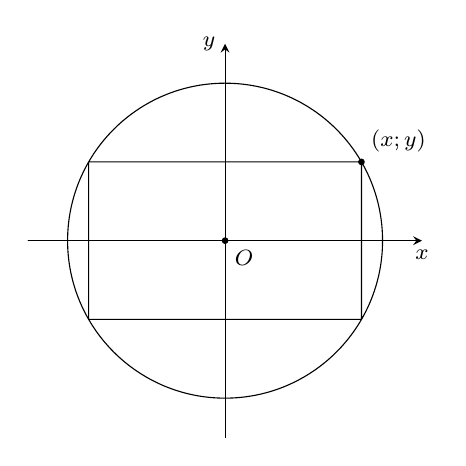
\begin{tikzpicture}[scale=1, font=\footnotesize, line cap=round, line join=round, >=stealth]
\def\r{2}
\path (0,0)coordinate(O)+(30:\r)coordinate(A)+(150:\r)coordinate(B)+(210:\r)coordinate(C)+(-30:\r)coordinate(D);
\draw[->] (-\r-.5,0)--(\r+.5,0)node[below]{$x$};
\draw[->] (0,-\r-.5)--(0,\r+.5)node[left]{$y$};
\draw (O)circle(\r cm) (A)--(B)--(C)--(D)--cycle;
\draw[fill=black] (0,0)node[below right]{$O$}circle(1pt) (A)node[above right]{$(x;y)$}circle(1pt);
\end{tikzpicture}
}
\noindent
Ta có $S(0) = 0$; $S(4) = 0$; $S(2\sqrt{2}) = 32$.\\
Vậy cửa sổ hình chữ nhật lớn nhất nội tiếp đường tròn có bán kính $4$ sẽ là hình vuông với diện tích $32$, chiều dài và chiều rộng bằng $2\sqrt{2} \cdot 2 = 4\sqrt{2}$ (từ $2x$ và $2y$ với $x=y=2\sqrt{2}$).
}
\end{ex}
\TL
\begin{ex}%[0D8H3-2]
Hãy khai triển biểu thức $(2x-1)^5$.
\loigiai{
Ta có
\begin{align*}
(2x-1)^5 &= \mathrm{C}^0_5 (2x)^5 + \mathrm{C}^1_5 (2x)^4 (-1) + \mathrm{C}^2_5 (2x)^3 (-1)^2 + \mathrm{C}^3_5 (2x)^2 (-1)^3 + \mathrm{C}^4_5 (2x) (-1)^4 + \mathrm{C}^5_5 (-1)^5\\
&=2^5 \cdot x^5 + 5\cdot 2^4 \cdot x^4 \cdot (-1) + 10 \cdot 2^3 \cdot x^3 \cdot 1 + 10 \cdot 2^2 \cdot x^2 \cdot (-1) + 5 \cdot 2x \cdot 1 + (-1)\\
&=32x^5 - 80x^4 + 80 x^3 - 40 x^2 + 10x - 1.
\end{align*}
}
\end{ex}

\begin{ex}%[0D8V2-4]%[Dự án đề kiểm tra Toán 10 HKII NH23-24- Trung Anh]%[THPT Việt Đức - Hà Nội]
Có $5$ bạn nam và $4$ bạn nữ được xếp vào một ghế dài có $9$ chỗ ngồi. Hỏi có bao nhiêu cách xếp sao cho bạn nam và nữ ngồi xen kẽ nhau?
\loigiai{
Giả sử các vị trí trên ghế dài được cho như sau
\[1\,\,\,\,2\,\,\,3\,\,\,4\,\,\,5\,\,\,6\,\,\,7\,\,\,8\,\,\,9\]
Để các bạn nam và nữ ngồi xen kẽ nhau thì khi và chỉ khi
\begin{itemize}
\item Nam được xếp vào vị trí số lẻ;
\item Nữ được xếp vào vị trí số chẵn.
\end{itemize}
Khi đó
\begin{itemize}
\item Số cách sắp xếp $5$ bạn nam vào $5$ vị trí mang số lẻ là $5!$
\item Số cách sắp xếp $4$ bạn nữ vào $4$ vị trí mang số chẵn là $4!$
\end{itemize}
Tổng số cách sắp xếp thỏa mãn điều kiện đề bài là \[5!\cdot 4!=2880\, (\text{cách}).\]
}
\end{ex}

\begin{ex}%[0H9V4-5]
Trong mặt phẳng với hệ trục tọa độ $Oxy$, cho đường tròn \[(C)\colon x^2+y^2+4x-2y-20=0\] và đường thẳng $\Delta\colon 3x+4y-m=0$. Tìm giá trị dương của tham số $m$ để đường thẳng $\Delta$ cắt đường tròn $(C)$ theo một dây dung có độ dài bằng $6$.
\loigiai{
\begin{center}
\begin{tikzpicture}[declare function={r=2.5;ga=40;},>=stealth,font=\scriptsize,scale=0.8]
%\path (0:0) coordinate (I)
%(ga:r) coordinate (A)
%(130:r) coordinate (B)
\coordinate (I) at (0,0);
\coordinate (A) at (ga:r);
\coordinate (B) at (130:r);
\coordinate (J) at ($(A)!1/2!(B)$);
\draw (I) circle (r)  ;
\draw (I)--(A)--(B)--(I)--(J);
\foreach \x/\g in{A/90,B/90,J/90,I/-90}
\fill[black](\x) circle (2pt)
($(\x)+(\g:5mm)$) node{\small $\x$};
\end{tikzpicture}
\end{center}
Đường tròn $(C)$ có tâm $I(-2;1)$ và bán kính $R=\sqrt{(-2)^2+1^2+20}=5$.\\
Giả sử $\Delta$ cắt $(C)$ tại hai điểm $A$ và $B$. Gọi $J$ là trung điểm của $AB$.\\
Khi đó $\heva{&IJ\perp AB\\&JB=\dfrac{1}{2}AB=3.}$\\
Xét tam giác $IJB$ vuông tại $J$ có $IJ=\sqrt{IB^2-JB^2}=4.$\\
Hay $\mathrm{d}(I; \Delta)=4$. Tương đương
\begin{align*}
&\dfrac{|(-2)\cdot3+4\cdot1-m|}{\sqrt{3^+4^2}}=4\\
\Leftrightarrow&\, |m+2|=4\cdot5=20\\
\Leftrightarrow&\, \hoac{&m+2=20\\&m+2=-20}\Leftrightarrow\hoac{&m=18\\&m=-22\,(\text{không thỏa mãn}).}
\end{align*}
Vậy $m=18$.
}

\end{ex}

